% Đầu sách: làm quen với Kriky. Không đánh số.

\chapter*{Làm quen với Kriky}
\addcontentsline{toc}{chapter}{Làm quen với Kriky}
\label{chuong:lam-quen}

Kriky là trợ lý giúp thầy cô ra đề kiểm tra trắc nghiệm, và giúp các em hiểu những câu mình làm sai.
Thầy cô nhắn cho Kriky bằng câu bình thường; Kriky soạn đề, thầy cô xem và duyệt. Chỉ thầy cô mới phát
hành được đề cho học sinh.

\section{Một bài kiểm tra đi qua những bước nào}

Hình~\ref{fig:vong-doi} cho thấy một bài kiểm tra đi từ lúc soạn tới lúc xem kết quả. Số trong mỗi ô
là thứ tự; dòng nhỏ dưới ô là chương nói về bước ấy.

\begin{figure}[htbp]
  \centering
  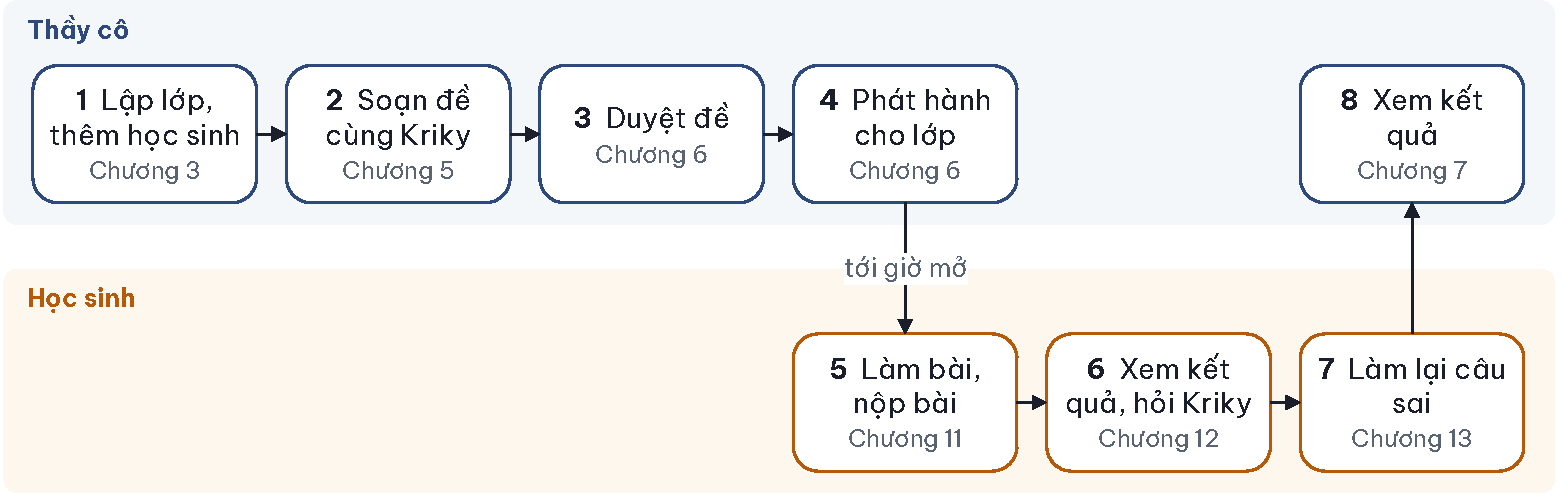
\includegraphics[width=\linewidth]{vong-doi-bai-kiem-tra.pdf}
  \caption[Vòng đời một bài kiểm tra]{Vòng đời một bài kiểm tra: thầy cô làm ở hàng trên, học sinh
    làm ở hàng dưới.}
  \label{fig:vong-doi}
\end{figure}

Bài làm có hai giai đoạn. Ở giai đoạn đầu, học sinh làm bài trong thời gian thầy cô đặt. Ở giai đoạn
hai, học sinh hỏi Kriky những câu mình sai, rồi làm một câu tương tự để gỡ điểm.

\section{Cần chuẩn bị gì}

\begin{bangtra}{L{3.6cm}Y}{\dau{Cần} & \dau{Chi tiết}}
  Máy tính & Màn hình máy tính hoặc laptop. Kriky được làm cho màn hình máy tính; trên điện thoại
  rất khó dùng. \\
  Trình duyệt & Chrome hoặc Edge bản mới. \\
  Địa chỉ trang giáo viên & \diachigiaovien \\
  Địa chỉ trang học sinh & \diachihocsinh \\
  Tài khoản giáo viên & Người quản lý Kriky của trường cấp (Chương~\ref{chuong:dang-nhap-gv}). \\
  Tài khoản học sinh & Thầy cô tạo cho cả lớp, rồi phát tên đăng nhập và mật khẩu cho từng em. \\
\end{bangtra}

\luuy{Thầy cô và các em dùng hai địa chỉ khác nhau. Học sinh vào nhầm trang giáo viên thì sẽ không đăng
nhập được bằng tên đăng nhập học sinh.}

\section{Bản Kriky đang dùng}

Góc trái dưới màn hình có tên bản, ví dụ \nhan{\tenban}. Sách này viết cho bản ấy. Khi cần báo lỗi,
bấm vào tên bản để chép lại (app không báo gì khi chép), rồi gửi kèm lời báo cho người quản lý Kriky
của trường.
